\documentclass{beamer}
\usetheme{Boadilla}
\usepackage{tikz}
\usepackage{graphicx}
\usepackage{animate}

\title{Weekly Presentation}
\subtitle{Week 38}
\author{}
\institute{Luleå University of Technology}
\date{\today}



\begin{document}
\begin{frame}
    \titlepage
\end{frame}


%%%%%%%%%%%%%%%% new page %%%%%%%%%%%%%%%%%%%%%%


\begin{frame}
    \subsection{Group members}
    \frametitle{Group members }
    \begin{itemize}
        \item Y-students
        \begin{itemize}
            \item Martin Blaszczyk - Project leader and object detection
            \item Edward Cedergård -Arm and gripping tool
            \item Niklad Dahlqvist -  Arm and gripping tool
            \item Måns Norell - Movable base
        \end{itemize}
        \item D-students
        \begin{itemize}
            \item Edward Källstedt - Object detection
            \item Albin Martinsson - Arrowhead and Git
        \end{itemize}  
    \end{itemize}
\end{frame}


%%%%%%%%%%%%%%%% new page %%%%%%%%%%%%%%%%%%%%%%


\begin{frame}{Robotic arm}
What we have done and what we are working on:
    \begin{itemize}
        \item Servos
        \item Representation (DH-parameters)
        \item Kinematics
        \item Chosen arm, 4DOF
        \item 3D modeling
    \end{itemize}
\end{frame}


%%%%%%%%%%%%%%%% new page %%%%%%%%%%%%%%%%%%%%%%


\begin{frame}{Servos}

    \begin{columns}
        \begin{column}[]{0.5\textwidth}
            \begin{itemize}
                \item Dynamixel
                \begin{itemize}
                    \item Feedback; position, torque, temperature, etc
                    \item Serial communication
                    \item Chainable
                \end{itemize}
            \end{itemize}
        \end{column}
        
        
        \begin{column}[]{0.5\textwidth}
            \begin{figure}
                \centering
                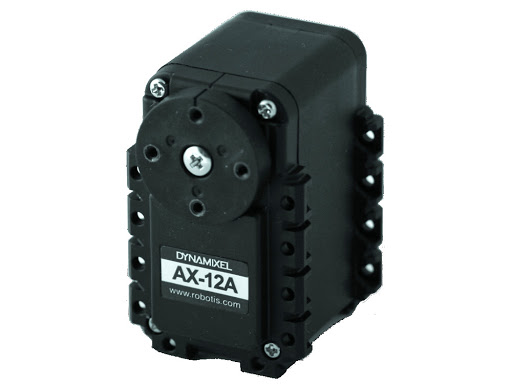
\includegraphics[width = \textwidth]{img/ax12a.jpg}
                \caption{Dynamixel AX-12A servo.}
            \end{figure}
            
        \end{column}
    \end{columns}
    
\end{frame}


%%%%%%%%%%%%%%%% new page %%%%%%%%%%%%%%%%%%%%%%


\begin{frame}{Representation}

    \begin{columns}
        \begin{column}[]{0.5\textwidth}
            \begin{itemize}
                \item Denavit–Hartenberg parameters
                \item Joints
                \item Degrees of freedom
            \end{itemize}
        \end{column}
        
        
        \begin{column}[]{0.5\textwidth}
            \begin{table}
                \begin{tabular}{l | c | c | c | c }
                Link & a & alpha & d & theta \\
                \hline \hline
                   1 & 0   & -90 & d1 & theta 1\\
                    2 & a2& 0 & 0 & theta 2\\
                    3  & a3 & 0 & 0& theta 3\\
                    4 & a4 & 0 & 0 & theta 4\\
                \end{tabular}
            \end{table} 
        \end{column}
    \end{columns}
    
\end{frame}


%%%%%%%%%%%%%%%% new page %%%%%%%%%%%%%%%%%%%%%%


\begin{frame}{Kinematics}

    \begin{itemize}
        \item Forward kinematics
        \item Inverse kinematics
        \item Numerical or analytical solution
        \item Robotics Toolbox in Matlab by Peter Corke
    \end{itemize}

    
\end{frame}


%%%%%%%%%%%%%%%% new page %%%%%%%%%%%%%%%%%%%%%%


\begin{frame}{Kinematics}
    \begin{figure}
        \centering
        \animategraphics[loop,width=0.7\linewidth]{12}{img/animation/00}{0}{74}
        \caption{3DOF robot moving in a triangle pattern.}
    \end{figure}
\end{frame}


%%%%%%%%%%%%%%%% new page %%%%%%%%%%%%%%%%%%%%%%

\begin{frame}{Chosen arm}

    \begin{columns}
        \begin{column}[]{0.5\textwidth}
            \begin{itemize}
                \item Four degrees of freedom
                \item 3DOF for positioning and \\
                a "wrist" for controlling the \\
                angle of the end effector
            \end{itemize}
        \end{column}
        
        
        \begin{column}[]{0.5\textwidth}
            \begin{figure}
                \centering
                \hspace*{-0.2\textwidth}
                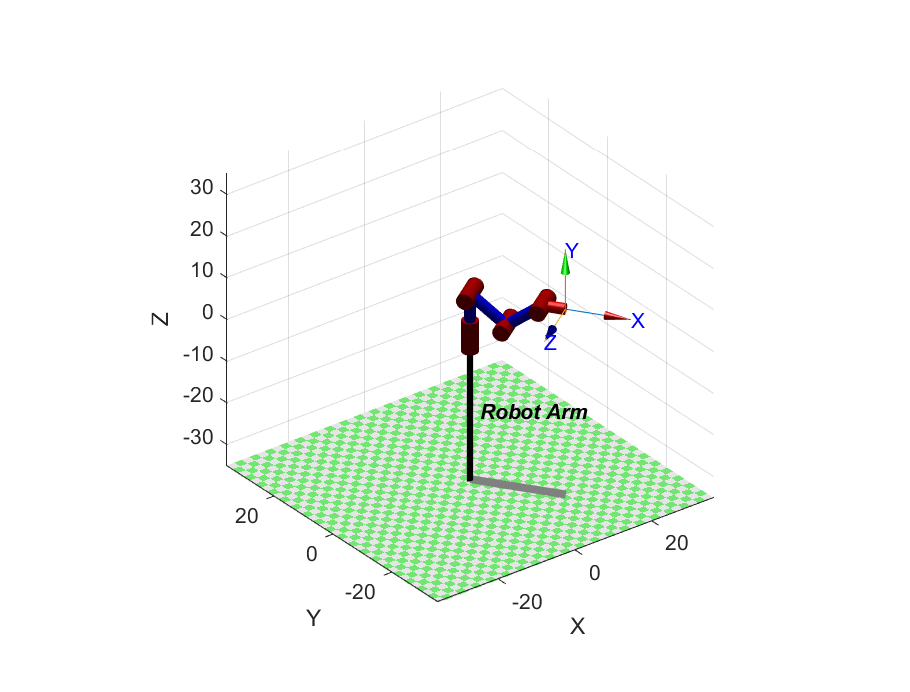
\includegraphics[width = 1.4\textwidth]{img/robotarm.eps}
                \caption{Representation of the robotic arm.}
            \end{figure}
            
        \end{column}
    \end{columns}
\end{frame}

%%%%%%%%%%%%%%%% new page %%%%%%%%%%%%%%%%%%%%%%


\begin{frame}{3D Modeling}

    \begin{itemize}
        \item Modeling in fusion 360
        \item Work in progress
        \item Time table
    \end{itemize}
\end{frame}


%%%%%%%%%%%%%%%% new page %%%%%%%%%%%%%%%%%%%%%%


%%%%%%%%%%%%%%%% new page %%%%%%%%%%%%%%%%%%%%%%


%%%%%%%%%%%%%%%% new page %%%%%%%%%%%%%%%%%%%%%%




%%%%%%%%%%%%%%%%%%%%%%%%%%%%%%%%%%%%%%%%%%%%%%%%%%%%%%%%%%%%%%%%
%%%%%%%%%%%%%%%%%%%%%%%% Time Plan %%%%%%%%%%%%%%%%%%%%%%%%%%%%%
%%%%%%%%%%%%%%%%%%%%%%%%%%%%%%%%%%%%%%%%%%%%%%%%%%%%%%%%%%%%%%%%
\begin{frame}
    \subsection{Time plan}
    \frametitle{Overall timetable}
    \begin{table}
        \begin{tabular}{| l | c | c | c | c }
            
            Sep & Oct & Nov & Dec \\
            \hline \hline
            Concept generation & Evaluation & Evaluation &  \\ 
            \hline
            Theory & Prototyping & Evaluation & Finishing up \\
            \hline
            Simulation & Evaluation & Evaluation & \\
            \hline
            Prototyping & Final Design & Evaluation &  \\
            \hline
 
        \end{tabular}
    \end{table}    
\end{frame}


\begin{frame}
    \frametitle{Time plan for September}
    \begin{table}
        \begin{tabular}{l | c | c | c | c }
        Subproject & Week 1 & Week 2 & Week 3 & Week 4 \\
        \hline \hline
            Arrowhead & Reading& Setup & API & Prototyping\\
            Movable base & Reading& Modeling & Simulation & Implementation\\
            Arm and grip  & Reading & Kinematics & Simulation& Prototyping\\
            Object detection & Reading & Testing & Prototyping & Evaluation\\
        \end{tabular}
    \end{table}
\end{frame}


\begin{frame}
    \begin{center}
        \Huge Questions?
    \end{center}
\end{frame}



\end{document}